\documentclass[10pt,a4paper]{article}

\newcommand{\COLORSDIR}{/Users/hoolywear/Desktop/UNIMORE/II ANNO/II SEMESTRE/colors}

\usepackage[italian]{babel}
\usepackage[usenames,dvipsnames]{xcolor}
\usepackage[utf8]{inputenc}
\usepackage[T1]{fontenc}
\usepackage{soul}
\usepackage[a4paper, portrait, margin=2.5cm]{geometry}
\usepackage{array}
\usepackage{tabularx}
\usepackage{multicol}
\usepackage{amsmath}
\usepackage{amsfonts}
\usepackage{amssymb}
\usepackage{algorithmicx}
\usepackage[noend]{algpseudocode}
\usepackage{wrapfig}
\usepackage{graphicx}
\graphicspath{ {./images/} }

\definecolor{emp}{HTML}{f9e9ec}
\definecolor{war}{HTML}{f88dad}
\definecolor{def}{HTML}{fac748}
\definecolor{the}{HTML}{1d2f6f}
\definecolor{obs}{HTML}{8390fa}


\usepackage{listings}

\definecolor{codeblue}{HTML}{074099}
\definecolor{codepurple}{HTML}{850075}
\definecolor{codered}{HTML}{98000f}

\lstdefinestyle{code}{
    backgroundcolor=\color{gray!10},   
    basicstyle=\ttfamily,
    breakatwhitespace=false,         
    breaklines=true,                 
    captionpos=b,                    
    keepspaces=true,                 
    showspaces=false,                
    showstringspaces=false,
    showtabs=false,                  
    tabsize=2,
    mathescape=true %dollar signs act as inline math delimiters
}
\lstdefinestyle{sql}{
    style=code,
    language=SQL,
    commentstyle=\color{codeblue},
    keywordstyle=\color{codepurple},
    stringstyle=\color{codered}
}

\lstset{style=sql}

\usepackage{mdframed}

% styles
\def\Clinewidth{.8pt}
\mdfdefinestyle{titlerule}{%
  frametitlerule=true,roundcorner=5pt,%
  frametitlerulewidth=\Clinewidth,%
  subtitleaboveline=true,subtitlebelowline=true,%
  subtitleabovelinewidth=\Clinewidth,subtitlebelowlinewidth=\Clinewidth,%
subtitlebackgroundcolor=obs,linewidth=1pt}
\mdfdefinestyle{emphasize}{%
  style=titlerule,%
  frametitle=,%
  linecolor=gray!50,linewidth=3pt,backgroundcolor=gray!10,%
  topline=false,bottomline=false,rightline=false}

% verbatim environment
\surroundwithmdframed[backgroundcolor=gray!5,hidealllines=true,%
                      innerleftmargin=1pt,innerrightmargin=1pt%
                      frametitle={}]{verbatim}

% algorithmic environment
\surroundwithmdframed[backgroundcolor=gray!10,hidealllines=true,%
frametitle={}]{algorithmic}

% quote environment
\surroundwithmdframed[style=emphasize]{quote}

% example environment
\newmdenv[frametitle=Esempio,style=titlerule]{example}

% definition environment
\newmdenv[frametitle=Definizione,style=titlerule,%
          linecolor=def]{definition}

% theorem environment
\newmdenv[frametitle=Teorema,style=titlerule,%
          linecolor=the]{theorem}

% emphasize environment
\newmdenv[style=emphasize,%
          linecolor=emp!70!red,backgroundcolor=emp]{emphasize}

% observation environment
\newmdenv[frametitle=Osservazione,%
          backgroundcolor=white,linecolor=obs,%
          frametitlebackgroundcolor=obs]{observation}

% warning environment
\newmdenv[style=emphasize,%
          backgroundcolor=war!10,linecolor=war]{warning}

\author{Iacopo Ruzzier}
\date{Ultimo aggiornamento: \today}


\title{%
Protocolli e Architetture di Rete\\
\large Appunti di laboratorio}

\begin{document}
\maketitle
\tableofcontents
\newpage
\section*{Marionnet}
\addcontentsline{toc}{section}{Marionnet}

\noindent
\begin{minipage}[c]{.5\textwidth}
Software per la simulazione di reti di calcolatori che offre un frontend grafico, basato su UML e altri tools, includendo
\begin{itemize}
  \item host di rete
  \item hub e switch
  \item router
  \item gateway Internet
\end{itemize}
\end{minipage}
\hfill
\begin{minipage}[c]{.3\textwidth}
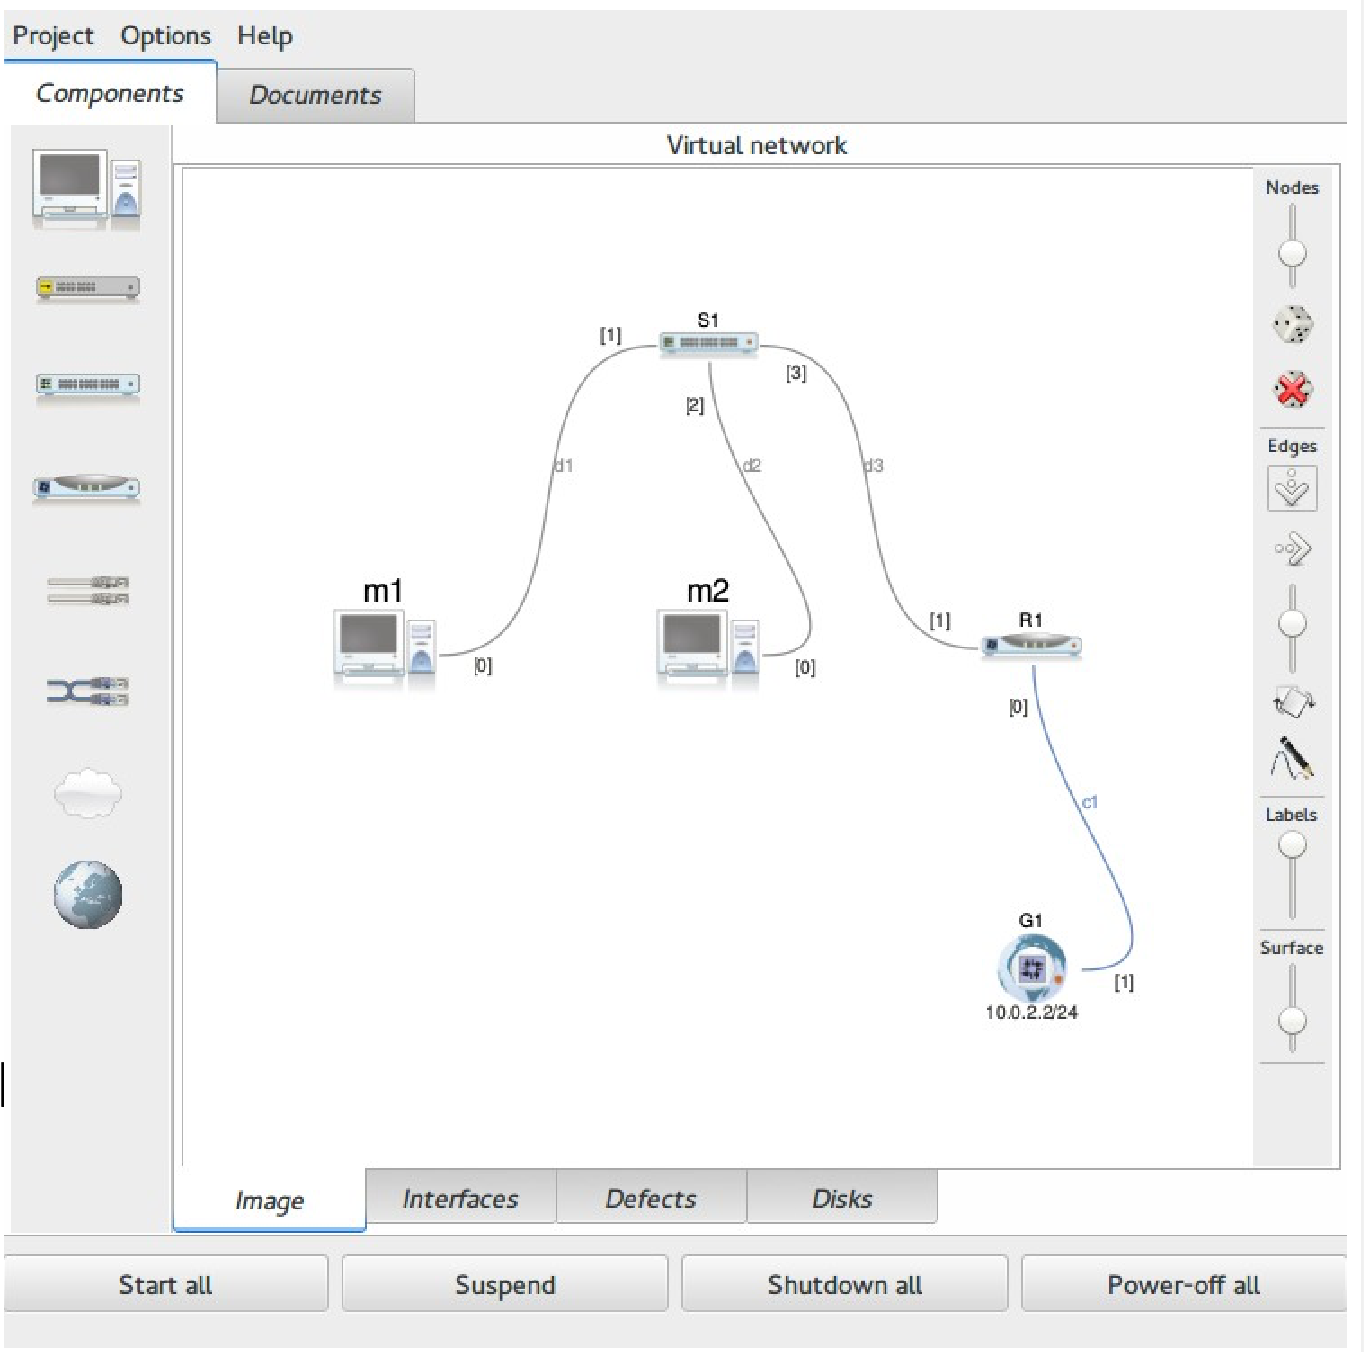
\includegraphics[width=\textwidth]{marionnet_intro_img.png}
\end{minipage}

\subsection*{Utilizzo durante il corso}
\addcontentsline{toc}{subsection}{Utilizzo durante il corso}

Tramite VM remote FIM, o installando il sistema in locale dai link su Moodle

Si consiglia l'uso del sistema \lstinline|aapar2|

\begin{warning}
    Per il momento i sistemi presenti nei laboratori e nelle distribuzioni \textbf{non sono compatibili tra loro}
\end{warning}

\subsection*{Nuovo progetto e configurazione base}
\addcontentsline{toc}{subsection}{Nuovo progetto e configurazione base}

\lstinline|Project -> New| e ci ritroviamo sulla schermata iniziale del nuovo workspace\\
Per inserire una nuova macchina, usiamo l'icona a sinistra oppure \lstinline|Ctrl + M|. Nel menu a comparsa abbiamo la possibilit\`a di modificare

\noindent
\begin{minipage}[c]{.5\textwidth}
\begin{itemize}
  \item \lstinline|name|: deve essere univoco nel network
  \item \lstinline|label|: descrizione opzionale
  \item \lstinline|memory|: la RAM (tipicamente 100MB o pi\`u)
  \item \lstinline|ethernet cards|: numero di schede ethernet
  \item \lstinline|distribution|: usiamo \lstinline|aapar2|, creata dal prof per il corso
  \item \lstinline|variant|: modifiche persistenti alla macchina
  \item \lstinline|kernel|: usiamo \lstinline|aapar2|
\end{itemize}
\end{minipage}
\hfill
\begin{minipage}[c]{.2\textwidth}
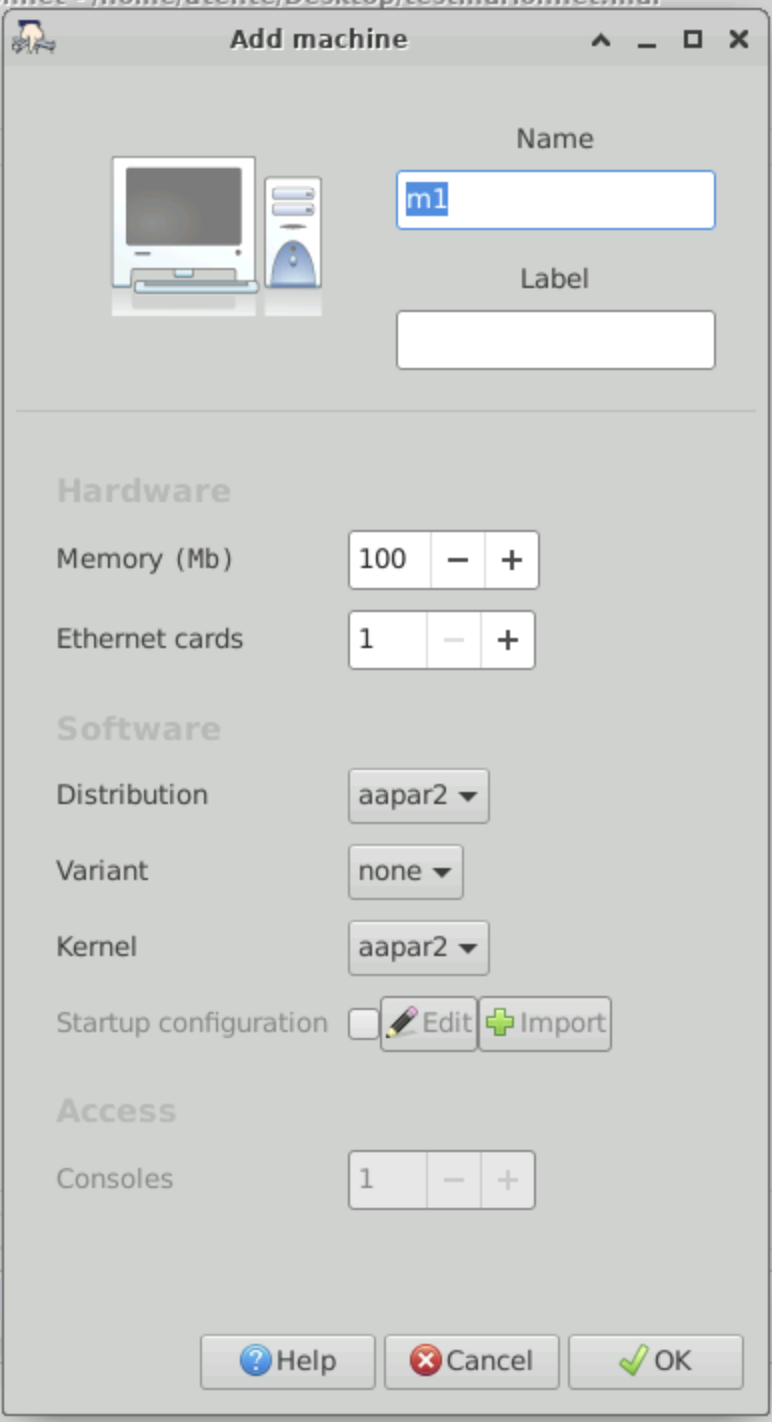
\includegraphics[height=150px]{marionnet_add_machine.png}
\end{minipage}


\subsection*{Cavi}
\addcontentsline{toc}{subsection}{Cavi}

\begin{itemize}
  \item cavi \textbf{crossover} (incrociati): connessioni tra dispositivi di rete dello \textbf{stesso livello dello stack}
  \item cavi \textbf{straight} (dritti): connessioni tra disp. di livello differente
\end{itemize}

\begin{example}[frametitle={Esempio base: collegare due macchine tra loro}]
  Creo due macchine e le collego mediante crossover cables. Per attivare le shell delle macchine, clicchiamo su \lstinline|Start all|
\end{example}


\end{document}
